%%%%%%%%%%%%%%%%%%%%%%%%%%%%%%%%%%%%%%%%%%%%%%%%%%%%%%%%%%%%%%%
% Welcome to your epic template on overleaf :)
% This part is just preamble stuff.
% Head down to where it says "Start here"
%%%%%%%%%%%%%%%%%%%%%%%%%%%%%%%%%%%%%%%%%%%%%%%%%%%%%%%%%%%%%%%

\documentclass[11pt]{article}

\usepackage[margin=1in]{geometry} % adjust margins and stuff
\usepackage{amsmath,amsthm,amssymb} % math symbols
\usepackage[dvipsnames]{xcolor} % text coloring
\usepackage{parskip}[skip = 10pt, indent = 0pt] % paragraph indentation and spacing
\usepackage{empheq} % boxes around answers
\usepackage{wrapfig} % wrap pictures with text
\usepackage{subfig}
\usepackage{graphicx} % insert pictures
    \graphicspath{{./images/}}
\usepackage{hyperref} % to put links and stuff
    \hypersetup{
        colorlinks=true,
        linkcolor=blue,
        % filecolor=magenta,      
        urlcolor=cyan,
        % pdftitle={Overleaf Example},
        % pdfpagemode=FullScreen,
        }
\usepackage{witharrows} % awesome package for arrows alongside math
\usepackage{titlesec} % change title formatting
    \titleformat{\section}
        {\Large\scshape\raggedright} % format
        {\thesection} % section name
        {7pt} % sep
        {} % before-code
        [{\titlerule[0.4pt]}] % after-code{}
    \titleformat{\subsection}
        {\normalsize\bf\scshape\raggedright} % format
        {\thesubsection} % section name
        {7pt} % sep
        {} % before-code
        [] % after-code{}
\usepackage[]{multicol}
\usepackage{fancyhdr} % headers and footers stuff
\usepackage{indentfirst} % indent first paragraph of sections
\usepackage{caption}
     \captionsetup{%
      font={footnotesize}, % small font size
      labelfont={bf,sf},      % label in bold, sans-serif
      singlelinecheck=true, % centered single-lined captions
      format=plain,             % indention=1cm,
      labelsep={colon},         % default separator: none, colon, period, space, quad, newline, endash
      hypcap = false, % avoid hyperlink warning
      width = 200pt
      }
\usepackage{minted} % pretty code
\usepackage[nodayofweek]{datetime} % generate current date and stuff
\usepackage{lipsum} % useful to generate text blocks

\newcommand{\N}{\mathbb{N}} % Natural numbers
\newcommand{\Z}{\mathbb{Z}} % integers
\newcommand{\inch}{\ensuremath{\,\textrm{in.}}} % use "in." in math mode
\newcommand{\dif}{\ensuremath{\,\textrm{d}}} % use d in math mode (derivatives & int)
\newcommand*\widefbox[1]{\fbox{\hspace{1em}#1\hspace{1em}}} % make boxes around answers

\newenvironment{ex}[2][Exercise]{\begin{trivlist}
    \item[\hskip \labelsep {\bfseries #1}\hskip \labelsep {\bfseries #2}]}{\end{trivlist}}
\newenvironment{sol}{ \color{blue}{ } }

\def\quadratic#1#2#3{ \frac{ -(#2) \pm \sqrt{ (#2)^2-4(#1)(#3) } }{ 2(#1) } } % quadratic equation


\pagestyle{fancy}
\lhead{\rightmark}
\rhead{}
\setlength{\headheight}{19pt}
\lfoot{Brigham Young University}
\rfoot{ME 497R: Mentored Research}

\begin{document}
% --------------------------------------------------------------
%                         Start here
% --------------------------------------------------------------
% \thispagestyle{empty}
\centering
\LARGE{Wing Optimization - 497R}\\
\normalsize
\vspace{5pt} Samuel Nasman, BYU FLOW Lab \\
\vspace{5pt} \longdate \today \\


\vspace{10pt}

%%%%%%%%%%%%%%%%%%%%%%%%%%%%%%%%%%%%%%%%%%%%%%%%%%%%%%%%%%%%%%%%%%%%%
%%%%%%%%%%%%%%%%%%%%%%%%%%%%%%%%%%%%%%%%%%%%%%%%%%%%%%%%%%%%%%%%%%%
\begin{minipage}{14cm}
    \centering
    \textbf{Abstract - } \textit{Minimizing induced drag is a vital design consideration for aircraft efficiency. This paper explores the capabilities of a gradient-based optimizer to obtain an optimal chord-distribution provided a compatible set of constraints. Results are compared to an analytical solution. }
\end{minipage}

\rule{0.2\textwidth}{0.5pt} . \rule{0.2\textwidth}{0.5pt}

\begin{multicols}{2}

\raggedright
\section{Introduction and Methods}
\setlength{\parindent}{12pt}
The purpose of this exploration is to better understand how changing
geometric properties of a wing (particularly chord distribution)
affects a wing's aerodynamic properties, as illustrated by the 
outputs of the Vortex Lattice Method (VLM). Particularly, we will
explore solving an optimization problem that seeks to find the chord distribution
that minimizes induced drag given a set of constraints: \vspace{-10pt}

\begin{multicols}{2}
    \begin{itemize}
        \itemsep-6pt
        \item span = 8.0 m 
        \item $\alpha = 5^{\circ} $
        \item Lift $\geq$ 1.7 N 
        \item $V_{\infty} = 1$ m/s
        \item quarter chords are aligned
        \item zero twist
        \item zero sweep
        \item[]
    \end{itemize}
\end{multicols}
\vspace{-10pt}

For our analysis we will use Julia programming language. Of particular 
mention, the VortexLattice.jl package and SNOW.jl packages will be used,
both of which are developed by the BYU FLOW Lab. VortexLattice.jl will
be used to model the aerodynamics of a simple wing and SNOW.jl will be used as 
a wrapper for IPOPT's gradient-based interior-point optimization algorithm. \par

Additionally, the results will be compared to the analytical solution 
to this particular problem (see the 
\href{https://en.wikipedia.org/wiki/Supermarine_Spitfire}{Supermarine 
Spitfire}).

\section{Results and Discussion}
From study of the first chapter of ``Engineering Design Optimization" by Dr. Martin and 
Dr. Ning (notes \href{https://github.com/samiamandyesican/497R/wiki/Design-Optimization}{here}), 
we learn that it's critical to thoroughly understand
an optimization problem because an optimizers will take advantage of any weakness
in your logic. Optimization problems are of the form \vspace{0pt}
\begin{align*}
    \text{minimize }& f(x) \\
    \text{by varying }& \underline x_i \leq x_i \leq \bar x_i \\
    \text{subject to }& \underline g_i \leq g(x) \leq \bar g_i
\end{align*}

Where $x$ and $g(x)$ are generally vectors.
One other important note is that \textbf{the number of constraints must be 
less than or equal to the number of design variables}. We will now 
approach the given design problem using SNOW.jl as our gradient-based
optimizer.\par

\subsection{Wing Optimization}
For this particular problem we will be minimizing the induced drag, $D_i$,
by varying the chord distribution subject to a minimum lift of 1.7 N given other constants as parameters throughout the optimization process.\par

In other words, for our optimization, $f(x)$ is the induced drag, $x$ is the chord distribution, and $g(x)$ is the lift generated by the wing. All of the other parameters given in the problem statement are either independent of the chord distribution or unconstrained. \par

I set the bounds on $x$ to be $(0, \infty)$ and the bounds on $g(x)$ to be $[1.7, \infty)$. The lift can be obtained from the lift coefficient, CL, output by VortexLattice.jl's \texttt{body\_forces()} function. The following definition is necessary to obtain the dimensionalized lift:

\[
C_L = \frac{L}{\frac{1}{2}\rho u^2 S} \implies L = \frac{1}{2}\rho u^2 S C_L
\]

Where $\rho$ is 1.0 kg/$\text{m}^3$, $u$ is 1.0 m/s, and $S$ and $C_L$ are dependent on the chord distribution, $x$. $S$ is the area of the wing and is in m/s. The lift coefficient, $C_L$, is dimensionless. \par

Similarly, the induced drag is obtained by
\[
D = \frac{1}{2}\rho u^2 S C_D
\]

\vspace{-30pt}
Next, it is important to note that it is necessary for our analysis to include additional constraints to avoid generating solutions like the chord distribution in Figure 1.\par

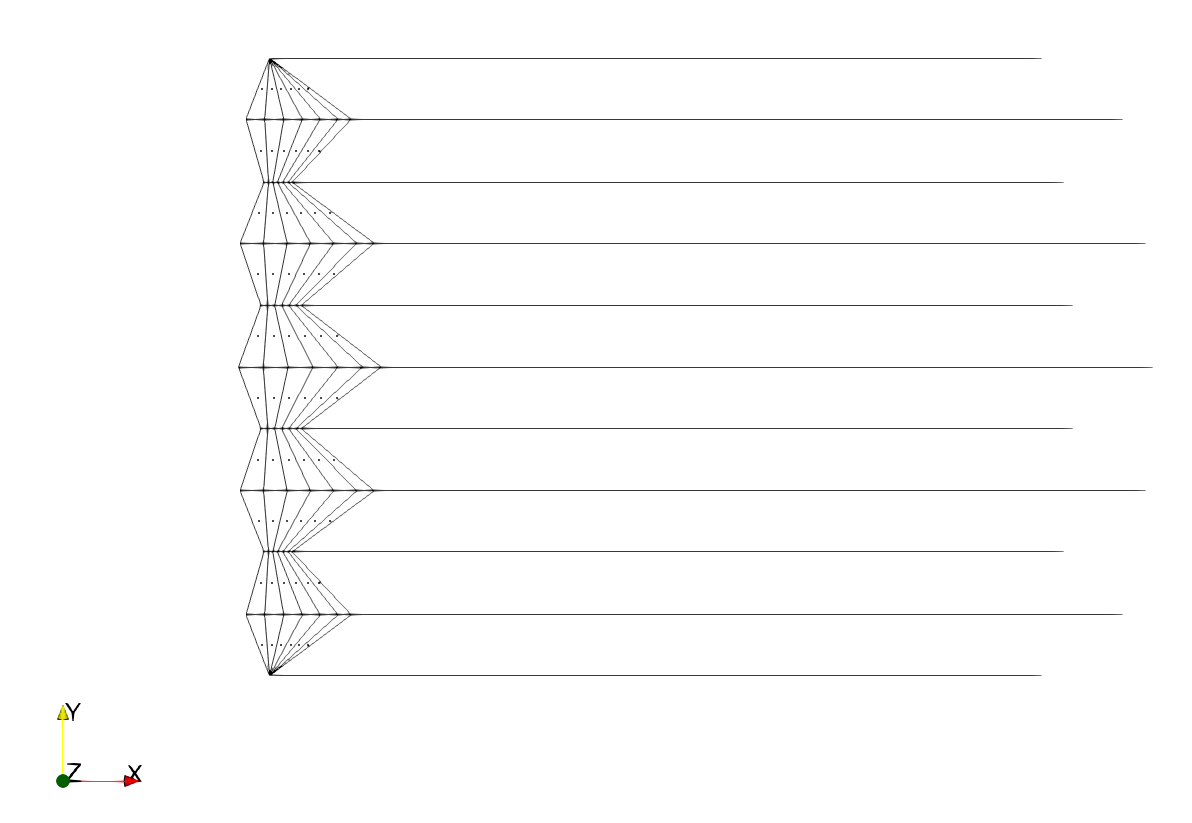
\includegraphics[width=0.90\linewidth]{images/vtk_unconstrained-test5x6.png}
    \captionof{figure}{Wing with chord distribution optimized to minimize induced drag, prior to enforcing chord monotonicity constraint.}
\vspace{10pt}
\hspace{12pt} It seems that there is some sort of pattern happening here, but I am not confident in explaining the exact reasons as to why the optimizer arrives at this solution. It is worth noting that this shape appears to be a noisier version of the final result we obtain. Because from a practical and structural point of view this result is sub-optimal, I will avoid this jagged behavior by implementing a monotonically decreasing constraint to $g(x)$ where each chord length (moving from root to tip) is required to be less than the previous chord length. This can be done using \texttt{diff($x$)}, which returns the difference between consecutive elements in a vector. The resulting optimization problem is: \par

\vspace{-5pt}
\begin{alignat*}{5}
    \text{minimize }& && && && f(\Vec{x}) && \\
    \text{by varying }& &&\Vec{0} &&< &\quad&\vec{x_i} &&< \Vec{\infty} \\
    \text{subject to }& &&1.7 &&\leq &&g[1](\vec{x}) &&< \infty \\
    & -&&\vec{\infty} &&< &&g[2:n](\vec{x}) &&< \vec{0}
\end{alignat*}

\noindent{Where $g[1](\vec{x})$ is the lift produced by the wing, $g[2:n](\vec{x})$} is the vector returned by \texttt{diff($x$)}, and $n$ is the length of the vector $\vec{x}$. In order to produce the desired monotonicity, $g[2:n]$ is constrained to be negative. \par

\setlength{\parindent}{12pt}
Note that we have $n$ chords in the $x$ vector and $n$ constraints in $g(x)$. This is acceptable since the number of constraints must be less than or equal to the number of design variables. Also note that the number of elements in $x$ is equal to one more than the number of span-wise panels that define the wing (called \texttt{ns} by VortexLattice.jl). \par 

Running the optimization with 4 span-wise panels (reflected across the root), 4 chord-wise panels, and an initial uniform chord distribution of 1.0 m results in Figure 2:

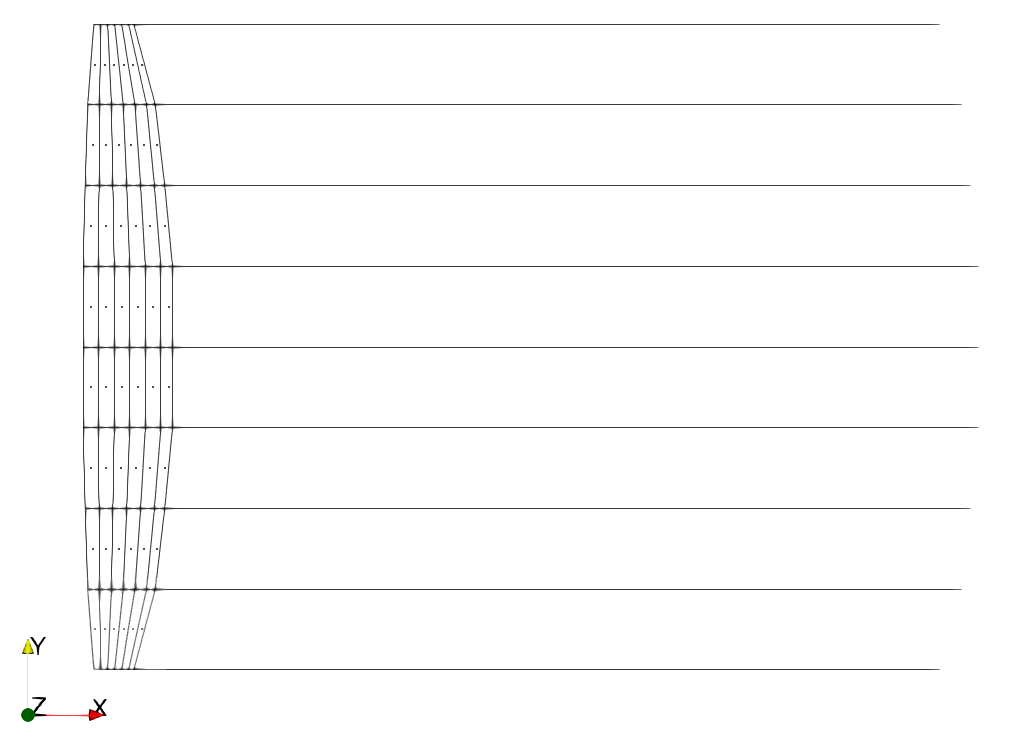
\includegraphics[width=0.90\linewidth]{images/4x6.png}
    \captionof{figure}{Wing optimization after including a monotonicity constraint.}

\vspace{10pt}
This chord distribution produces 0.0256 N of induced drag and 1.7 N of lift and is defined by the following vector (in meters):
\[ \vec{x} = 
\begin{bmatrix}
    1.158953937269707\\ 1.1589494398673357\\ 1.0321804324508204\\ 0.8813544247245128\\ 0.5191080277239004
\end{bmatrix}
\]

\setlength{\parindent}{12pt}
\subsection{Comparison to the Supermarine Spitfire}
This particular optimization problem (chord distribution to minimize induced drag) actually has an analytical solution that is utilized by the famous aircraft Supermarine Spitfire (Figure 6). It is based on the elliptic circulation distribution defined by:
\[
\Gamma(y) = \Gamma_0 \sqrt{1 - \left( \frac{y}{\frac{b}{2}} \right)^2}
\]
Where 
\[\Gamma_0 = \frac{2 u_{\infty}SC_L}{b\pi}.\]

By the fundamental lifting line equation, we can deduce that if this wing has a constant airfoil throughout (though not necessarily the same size throughout), the product $c(y)\alpha(y)$ must also be elliptic. Since we are looking at a wing with no twist, then the chord distribution $c(y)$ must also be elliptic (\textit{Engineering Design Optimization} 121-124).\par 

It is useful to compare the circulation distribution produced by our optimization to the analytical circulation distribution. The circulation distribution of our model can be obtained indirectly by the VortexLattice.jl function \texttt{lifting\_line\_coefficients()}, since one of its outputs is the 2-dimensional lifting-line coefficient $c_{\ell}$ for each of the lifting lines associated with the chord distribution.

By the Kutta-Joukowski Theorem lift per unit-span is given by:
\begin{align*}
    L' = \rho_{\infty} u_{\infty} \Gamma 
\end{align*}
And as noted earlier the definition of the lift coefficient gives
\[
L = \frac{1}{2}\rho u^2 S C_L \implies L' = \frac{1}{2w}\rho u^2 S c_{\ell}
\]
Where for a single panel the reference area $S = w\bar{c}$ and $w$ is the span-wise depth of the discretized airfoil with $\bar{c}$ as the mean chord of that panel. Therefore
\begin{align*}
    L' &= \rho_{\infty} u_{\infty} \Gamma = \frac{1}{2w}\rho u^2 (w \bar{c}) c_{\ell} \\
    & \implies \Gamma = \frac{1}{2}u_{\infty}\bar{c}c_{\ell}
\end{align*}

This formula is implemented in VLM\_functions.jl's \texttt{extract\_circulation()} and results in the comparison between the analytical and optimized solutions displayed in Figure 3. \vspace{7pt}

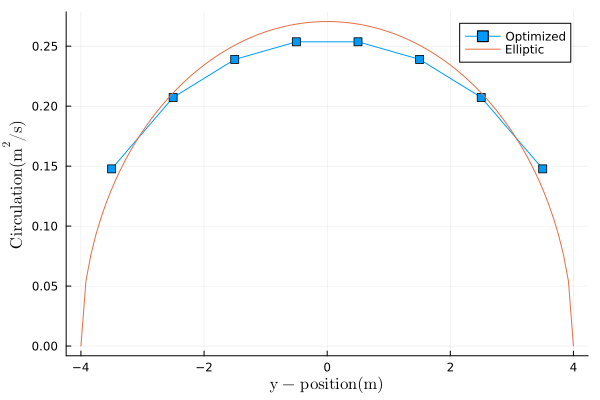
\includegraphics[width=0.90\linewidth]{images/test4x6.png}
    \captionof{figure}{Comparison of optimized circulation to theoretical elliptic circulation distribution for the wing in Figure 2. The error between the two distributions has $\sigma = 0.012818$ with a maximum of $12.9\%$.}

\vspace{7pt}
Increasing the number of panels gets us closer to the theoretical value as shown in Figure 4. Note that the maximum percent error between the two distributions is actually larger. This is most likely explained by the steepness of the curve towards the tips of the wings, with a higher-fidelity distribution having points closer to the tips.
\vspace{7pt}

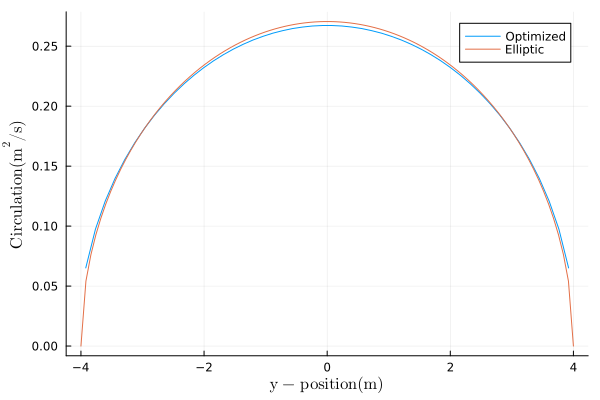
\includegraphics[width=0.90\linewidth]{images/test25x6.png}
    \captionof{figure}{Comparison of optimized circulation to theoretical elliptic circulation distribution for a wing with 6 chord-wise panels and 25 span-wise panels. The error between the two distributions has $\sigma = 0.003540$ with a maximum of $22.3\%$.}

\vspace{7pt}
Note the similarity of the optimized chord distribution (Figure 5) to the Supermarine Spitfire (Figure 6). 

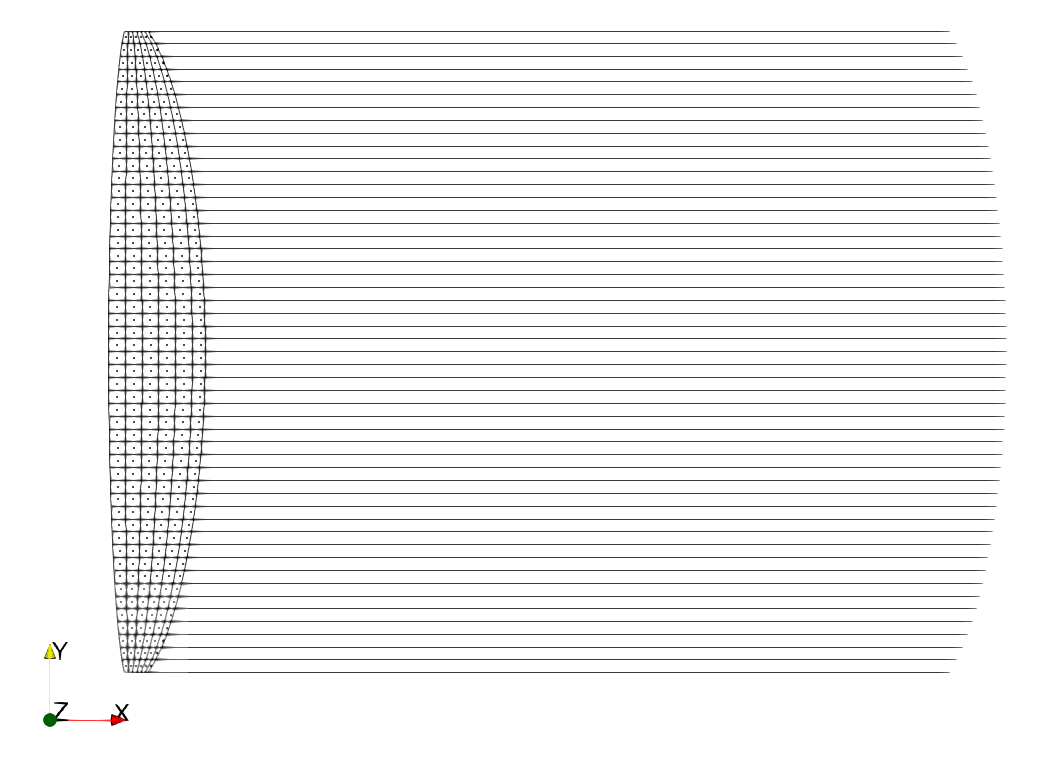
\includegraphics[width=0.90\linewidth]{images/25x6.png}
    \captionof{figure}{Chord distribution optimized to minimize induced drag. Composed of 25 span-wise panels and 6 chord-wise panels.}
\vspace{12pt}
\hspace{20pt}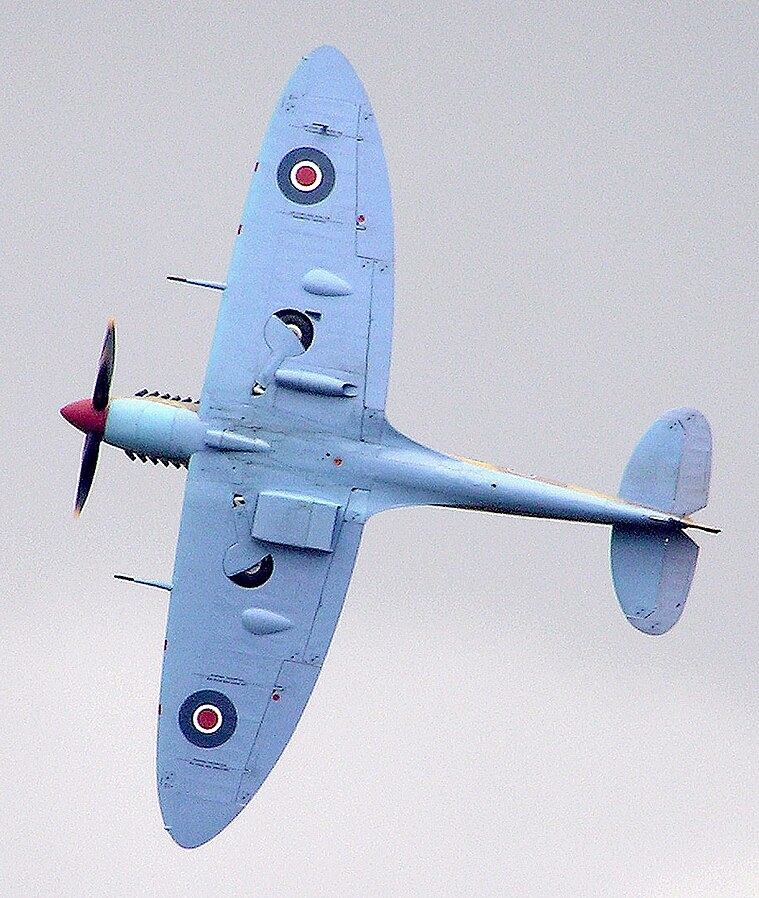
\includegraphics[width=0.70\linewidth]{images/spitfire-planform.jpg}
    \captionof{figure}{Supermarine Spitfire planform. Image from Adrian Pingstone, Wikimedia, public domain.}

Worthy of note from the 25x6 panel optimization is that it generates 0.0283 N of induced drag and 1.7 N of lift. This is actually \textit{more} induced drag than the 4x6 panel optimization (0.0256 N), which I find difficult to explain. This is an area for future exploration.

\section{Conclusion}
\setlength{\parindent}{12pt}
By numerical optimization, I found that for an untwisted monotonic wing the optimal chord distribution (from an induced drag point of view) is elliptic. The highest fidelity model that I generated for this particular optimization problem generates 1.7 N of lift and 0.0283 N of induced drag and is displayed in Figure 5. \par

Future exploration may be done to explore the reasons for the necessity of a monotonic constraint in order to obtain a smooth, elliptic distribution. Additionally, the cause of an increase in induced drag in response to increased fidelity may be explored. \par

Another area of research would be to explore the feasible space and possibly implement scaling to improve the optimization's efficiency and versatility. \par

Additionally, the number of design variables could be reduced by implementing splines to use a single variable to devine multiple panels. Sine-spacing could serve the same function, to increase fidelity near the wing-tip since the curve is so much steeper.\par

Other areas of future research include optimizing the twist distribution rather than the chord distribution and implementing a method for predicting stall, such as an interpolated look-up table. 

\section{References}
\noindent
Joaquim R.R.A. Martins and Andrew Ning. \\ \hspace{12pt} 
Engineering Design Optimization. \\ 
\hspace{12pt} Cambridge University Press, 2021. \\ 
\hspace{12pt} ISBN:n9781108833417. 
    
\end{multicols}

%%%%%%%%%%%%%%%%%%%%%%%%%%%%%%%%%%%%%%%%%%%%%%%%%%%%%%%%%%%%%%%%%%%%%%%%%%%%
% --------------------------------------------------------------
%     You don't have to mess with anything below this line.
% --------------------------------------------------------------

\end{document}